\documentclass[aspectratio=169,11pt]{beamer}
\usepackage[T1]{fontenc}
\usepackage{tgheros,booktabs,tikz,array}
\usetikzlibrary{arrows.meta,positioning}
\definecolor{ink}{HTML}{173044}
\definecolor{green}{HTML}{006F67}
\definecolor{mist}{HTML}{E8F4F1}
\definecolor{slate}{HTML}{516777}
\setbeamercolor{normal text}{fg=ink,bg=white}
\setbeamercolor{frametitle}{fg=ink}
\setbeamerfont{frametitle}{size=\LARGE,series=\bfseries}
\setbeamertemplate{navigation symbols}{}
\setbeamersize{text margin left=9mm,text margin right=9mm}
\setbeamercolor{title band}{fg=white,bg=ink}
\setbeamercolor{footer}{fg=ink,bg=mist}
\setbeamertemplate{frametitle}{%
  \nointerlineskip
  \begin{beamercolorbox}[wd=\paperwidth,leftskip=9mm,rightskip=9mm,sep=0pt]{title band}
    \vskip2.5mm\rightskip=9mm plus 1fil\usebeamerfont{frametitle}\insertframetitle\par\vskip2.5mm
  \end{beamercolorbox}}
\setbeamertemplate{footline}{%
  \begin{beamercolorbox}[wd=\paperwidth,ht=2.5ex,dp=1ex,leftskip=5mm,rightskip=5mm]{footer}
    \scriptsize
    \makebox[.32\paperwidth][l]{\fontsize{5}{6}\selectfont Pierpaolo Spadafora \enspace|\enspace Università della Calabria}%
    \makebox[.2975\paperwidth][c]{Lazy Heuristics in clingo}%
    \makebox[.32\paperwidth][r]{\insertframenumber\,/\,\inserttotalframenumber}
  \end{beamercolorbox}}
\newcommand{\accented}[1]{\textcolor{green}{\textbf{#1}}}
\tikzset{box/.style={draw=slate,rounded corners=2pt,minimum height=9mm,align=center,inner xsep=4mm}, flow/.style={-{Stealth},thick,draw=slate}}
\begin{document}
\begin{frame}[plain]
{\small University of Calabria \quad / \quad Master's Degree in Computer Science}\par
\vfill
{\huge\bfseries Lazy Declarative Heuristics in\\ Answer Set Programming\par}
\vspace{2mm}{\Large\color{green} Design and Evaluation of a clingo Propagator\par}
\vfill
{\large\bfseries Pierpaolo Spadafora}\par
{\small Student ID 263722}\par\medskip
\begin{columns}[T,onlytextwidth]
\begin{column}{.48\textwidth}
{\small\bfseries Supervisor at the University of Calabria}\par
{\small Prof. Carmine Dodaro}
\end{column}
\begin{column}{.48\textwidth}
{\small\bfseries Supervisors at the University of Potsdam}\par
{\small Prof. Dr. Torsten Schaub\\Dr. Javier Romero Dávila}
\end{column}
\end{columns}
\end{frame}

\begin{frame}{Grounding prepares every rule before search}
\centering
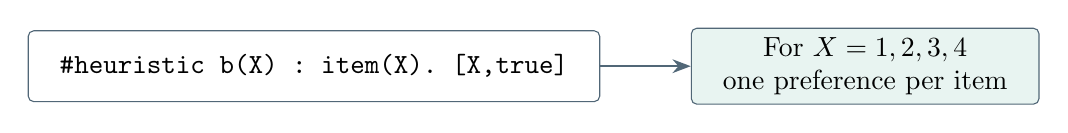
\begin{tikzpicture}
\node[box] (a) at (0,0) {\texttt{\#heuristic b(X) : item(X). [X,true]}};
\node[box,fill=mist] (b) at (7,0) {For $X=1,2,3,4$\\one preference per item};
\draw[flow] (a)--(b);
\end{tikzpicture}
\par\bigskip
\accented{Before search} the grounder prepares the heuristic directives the solver can use.
\par\medskip
\accented{During search} a lazy evaluator reads the current assignment and proposes the next choice.
\end{frame}

\begin{frame}[fragile]{A small heuristic can have a large grounding}
\centering
$N=\{1,2,3,4\}\qquad B=\{4\}\ (\text{sum }4)\qquad C=\{2,3\}\ (\text{sum }5)$
\par\medskip
\accented{Where should 1 go?}\quad Prefer $B$. Both groups then sum to 5.
\par\medskip
\raggedright\small
\begin{verbatim}
#heuristic b(X) : item(X), not c(X),
    S = #sum{Y : c(Y)}. [(n+1)*S+X, true]
#heuristic c(X) : item(X), not b(X),
    S = #sum{Y : b(Y)}. [(n+1)*S+X, true]
\end{verbatim}
\centering
The opposite group's sum determines the preference.
\par\bigskip
\begin{tabular}{rr}
$n=4$ & \accented{88 ground directives}\\
$n=100$ & \accented{1,010,200 ground directives}
\end{tabular}
\end{frame}

\begin{frame}{Native C++ updates the heuristic through \texttt{::Heuristic}}
\small \texttt{init} registers candidate literals and watches before search starts.
\par\bigskip
\centering
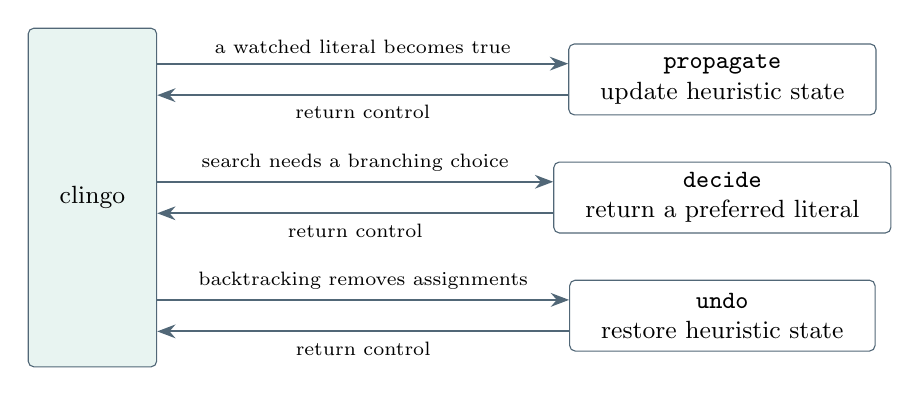
\begin{tikzpicture}[font=\small]
\node[box,fill=mist,minimum height=4.3cm] (solver) at (0,-1.5) {clingo};
\foreach \y/\name/\event/\action in {
0/propagate/a watched literal becomes true/update heuristic state,
-1.5/decide/search needs a branching choice/return a preferred literal,
-3/undo/backtracking removes assignments/restore heuristic state}{
\coordinate (s\name) at (solver.east |- 0,\y);
\node[box] (c\name) at (8,\y) {\texttt{\name}\\\action};
\draw[flow] ([yshift=2mm]s\name)--node[above,font=\scriptsize]{\event}([yshift=2mm]c\name.west);
\draw[flow] ([yshift=-2mm]c\name.west)--node[below,font=\scriptsize]{return control}([yshift=-2mm]s\name);
}
\end{tikzpicture}
\end{frame}

\begin{frame}{SWI-Prolog queries the trail at each decision}
\centering
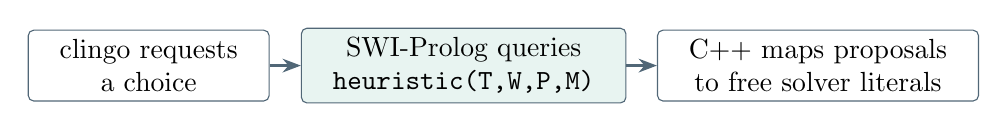
\begin{tikzpicture}
\node[box] (a) at (0,0) {clingo requests\\a choice};
\node[box,fill=mist] (b) at (4,0) {SWI-Prolog queries\\\texttt{heuristic(T,W,P,M)}};
\node[box] (c) at (8.5,0) {C++ maps proposals\\to free solver literals};
\draw[flow] (a)--(b);\draw[flow] (b)--(c);
\end{tikzpicture}\par\bigskip
Return the best eligible literal, or use clingo's fallback.
\end{frame}

\begin{frame}{Differences between semantics}
\small
\renewcommand{\arraystretch}{1.55}
\begin{tabular}{@{}>{\raggedright\arraybackslash}p{4cm}>{\raggedright\arraybackslash}p{4cm}>{\raggedright\arraybackslash}p{4cm}@{}}
 & \textbf{clingo-like} & \accented{Alpha-like}\\\midrule
\shortstack[l]{When does \texttt{not atom(X)}\\hold?} & \texttt{atom(X)} is established false & \texttt{atom(X)} is false or unassigned\\
$S=\#sum\{Y:c(Y)\}$ & Wait until the sum is fixed & Sum the currently true \texttt{c(Y)} atoms\\
$\#max$ with no true elements & $-\infty$ (\texttt{\#inf}) & $0$\\\bottomrule
\end{tabular}
\par\bigskip
\textbf{Example}\quad If \texttt{c(2)} is true and \texttt{c(3)} is unassigned,\\
Alpha-like evaluation uses $S=2$; clingo-like equality waits.
\end{frame}

\begin{frame}{Four ways to evaluate a heuristic}
\centering
\renewcommand{\arraystretch}{1.5}
\begin{tabular}{lcc}
 & \textbf{clingo-like} & \accented{Alpha-like}\\\midrule
Ground & \texttt{gc} & \texttt{ga}\\
Lazy & \texttt{lc} & \texttt{la}\\\bottomrule
\end{tabular}\par\bigskip
\raggedright Crossing two representations with two readings gives four variants in clingo.\\
We compare them with an unguided baseline and use Alpha as an external reference.
\end{frame}

\begin{frame}{BSP search drops to 120 choices}
\centering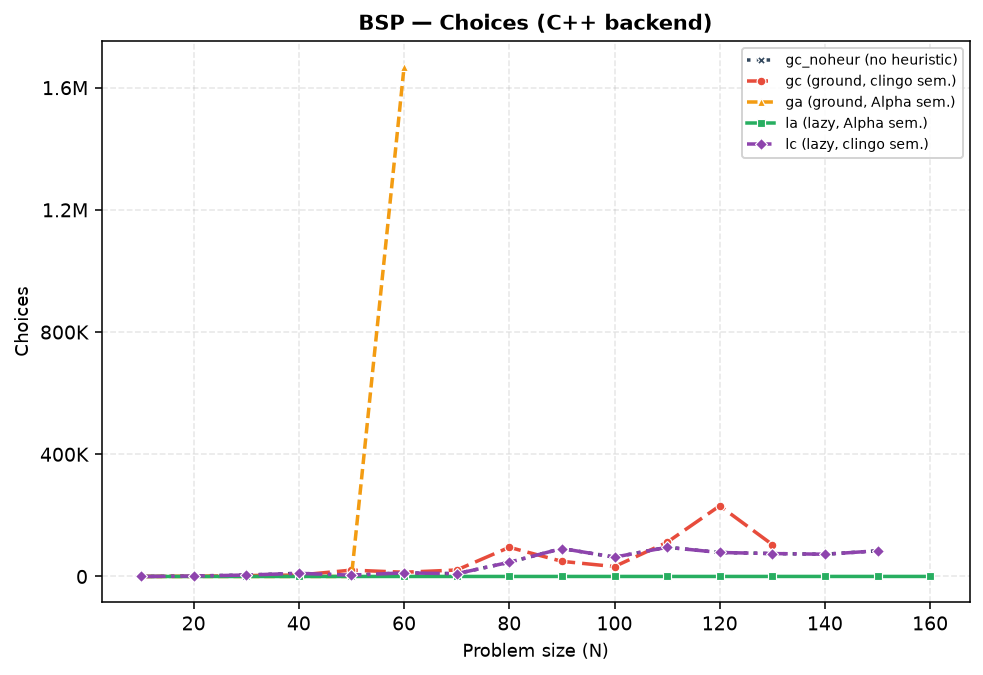
\includegraphics[height=.58\paperheight,width=.95\textwidth,keepaspectratio]{../thesis/Tesi_Lazy_Heuristics/figures/hpc/HD/bsp/native_choices.png}\par\medskip
At $n=120$, lazy Alpha-like guidance makes 120 choices with zero conflicts.
\end{frame}

\begin{frame}{PUP uses nearly half the time and memory}
\centering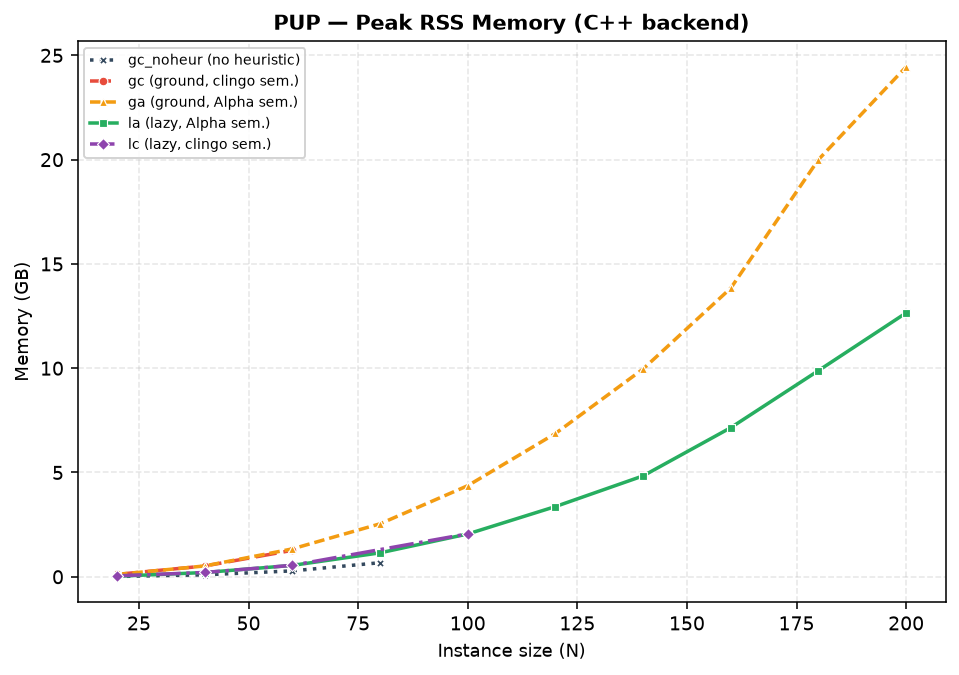
\includegraphics[height=.58\paperheight,width=.95\textwidth,keepaspectratio]{../thesis/Tesi_Lazy_Heuristics/figures/hpc/HD/pup/native_mem.png}\par\medskip
At $N=200$, peak memory falls from 24.4 to 12.7 GB and time from 438.6 to 224.0 s.
\end{frame}

\begin{frame}{Where does heuristic laziness pay off?}
\renewcommand{\arraystretch}{1.6}
\begin{tabular}{@{}lp{11.5cm}@{}}
\accented{BSP} & Even with 120 choices and zero conflicts, grounding the base program dominates runtime.\\
\accented{PUP} & Avoiding ground heuristic directives saves nearly half the peak memory on the largest instance.\\
\accented{HRP} & On house-20, Prolog spends about 94\% of its runtime in the propagator. The cost per decision matters.\\
\end{tabular}
\vfill
{\large\bfseries clingo can keep its ground-and-solve architecture and use the current assignment to guide each choice.}
\end{frame}
\end{document}
